\section{Surface} \label{sec:Surface}

Surface utility determines the average surface of structures such as
membranes or or polymer brushes.

The utility cuts the plane perpendicular to the chosen axis into squares of
size \texttt{<width>*<width>} and then finds the beads with the highest and
lowest coordinates along the chosen axis whose other two coordinates fall
into the square for each square on the plane. By default, it searches the
chosen axis for the beads with the highest coordinate in the interval
$\langle0, (box length)/2\rangle$ and with the lowest coordinate in the
interval $\langle(box\ length)/2; (box\ length)\rangle$, i.e., it assumes
something such as a polymer brush on each wall. If \texttt{-in}
option is used, it searches for a layer structure inside the box, i.e., it
searches for the bead with the lowest and highest coordinates in the whole
box, $\langle0; (box\ length)\rangle$ (this mode finds surfaces for
something like a bilayer).

Note that the utility does not determines any structures for now, therefore
any molecules outside the brush/membrane can be recognised as a part of the
surface (\texttt{-bt} and \texttt{-m} can be sometimes used to eliminate
this problem).

By default, all bead types and all molecule types are used, but using
\texttt{-bt} and \texttt{-m} options, only specified bead and/or molecule
types can be used. This is particularly useful when, e.g., other molecules
solubilise inside the brush/membrane, leaving some molecules in the
solution.

Following are two examples of usage with and without \texttt{-in} option
(on top are snapshots with coloured balls representing the detected surface
and on the bottom are graphs of the surface):

\begin{minipage}{0.45\textwidth}
  \centering
  \texttt{Surface in.vcf 1 out.txt z -in}
  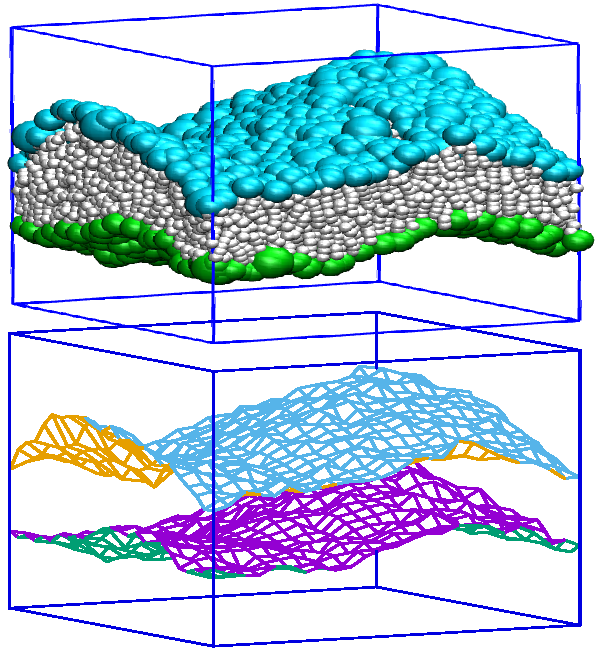
\includegraphics[width=\textwidth]{Surface-bilayer.pdf}
\end{minipage}
\hfill
\begin{minipage}{0.45\textwidth}
  \texttt{Surface in.vcf 1 out.txt z}
  \centering
  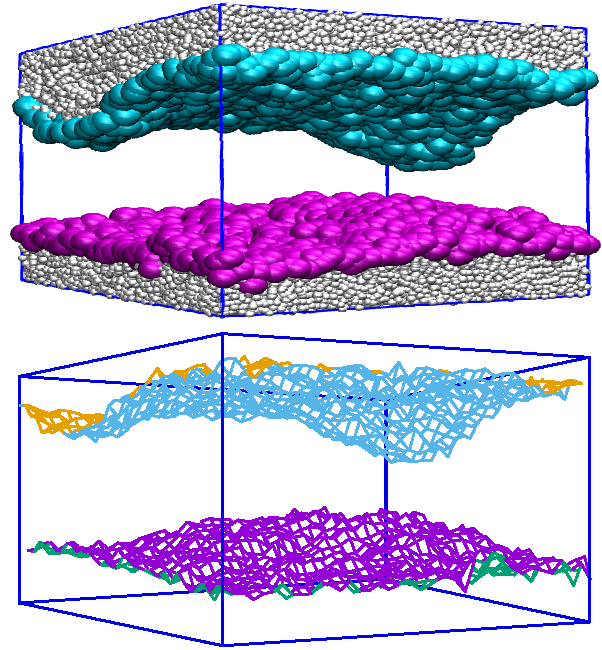
\includegraphics[width=\textwidth]{Surface-brush.pdf}
\end{minipage}

Usage:

\vspace{1em}
\noindent
\texttt{Surface <input> <width> <output> <axis> <options>}

\noindent
\begin{longtable}{p{0.2\textwidth}p{0.744\textwidth}}
  \toprule
  \multicolumn{2}{l}{Mandatory arguments} \\
  \midrule
  \texttt{<input>} & input coordinate file (either \texttt{vcf} or
    \texttt{vtf} format) \\
  \texttt{<width>} & side length of each square \\
  \texttt{<output>} & output file \\
  \texttt{<axis>} & direction in which to determine the surface: \texttt{x},
    \texttt{y}, or \texttt{z} \\
  \toprule
  \multicolumn{2}{l}{Non-standard options} \\
  \midrule
  \texttt{-in} & start from the box centre instead of from its edges \\
  \texttt{-m <name(s)>} & molecule type(s) to use (default: all) \\
  \texttt{-bt <name(s)>} & bead type(s) to use (default: all) \\
  \texttt{-st <int>} & starting timestep for calculation (default: 1) \\
  \texttt{-e <int>} & ending timestep for calculation (default: none) \\
  \bottomrule
\end{longtable}

\noindent
Format of output files:
\begin{enumerate}[nosep,leftmargin=20pt]
  \item \texttt{<output>} -- 3D coordinates
    \begin{itemize}[nosep,leftmargin=5pt]
      \item first line: command used to generate the file
      \item second line: column headers
        \begin{itemize}[nosep,leftmargin=5pt]
          \item first two numbers represent the centre of each square
            (being the coordinates on the sliced up plane); i.e., if \texttt{<width>} is 1,
            then the centre of the first square is 0.5 0.5, the centre of
            the second one is 0.5 1.5, etc.
          \item the second two numbers are coordinates of the surface in
            the third dimension, i.e., along the chosen axis
        \end{itemize}
    \end{itemize}
\end{enumerate}
